\chapter{Теоретическая часть}

\section{Условия проведения оилмпиады Ugra CTF}

Большую часть задач, связанных с проведением школьной олимпиады по защите информации Ugra CTF, можно автоматизировать.

В первую очередь, для этого необходимо разработать формальное описание задач с учётом специфики олимпиады Ugra CTF. Существует ряд требований, который необходимо удовлетворить: внутренние и внешние.

Источников внутренних требований несколько. К ним относятся официальные нормативные документы: положение об олимпиаде и регламент её проведения. Среди них наиболее важен регламент. Именно в нём описаны:

\begin{itemize}
\item порядок регистрации участников,
\item порядок проведения этапов олимпиады,
\item правила оформления и проверки работ,
\item порядок подведения итогов и др.
\end{itemize}

Эти требования составлены с учётом общих принципов проведения CTF-соревнований вида Jeopardy и уже написаны формальным языком. Кроме того, поскольку требования внутренние, их допустимо видоизменять.

Ко внешним требованиям относится «Порядок проведения олимпиад школьников», документ, написанный РСОШ и утверждённый приказом Министерства образования и науки РФ. Этот документ, в частности, описывает общие положения и то, как должна проходить олимпиада. Большая часть требований РСОШ уже включена во внутренный регламент проведения олимпиады, и эти требования видоизменять нельзя.

Следует отметить, что большая часть требований носит скорее юридический характер, и практически не устанавливает требования к технической инфраструктуре. Поэтому, их необходимо будет составить самостоятельно.

Кроме нормативно-правовых актов, регулирующих порядок проведения олимпиады и требования к участникам, существуют физические и технические ограничения, связанные с распределённо-очным форматом проведения олимпиады. Например, несмотря на сравнительную популярность CTF-соревнований, нельзя ожидать, что наблюдатели на площадках будут знакомы с особенностями этого формата и способны самостоятельно сконфигурировать подходящее сетевое и программное окружение для участников.

\subsection{Правила и порядок проведения олимпиады Ugra CTF}

Олимпиада состоит из двух этапов: отборочного (отбора, Ugra CTF Quals) и заключительного (финала, Ugra CTF School).

Отборочный этап проводится в дистанционном формате и состоит из двух зачётов. К участию в официальном зачёте допускаются обучающиеся школ и средне-специальных учебных организаций (колледжей, училищей и т.д.). Неофициальный зачёт открыт для всех желающих без ограничений, но такого права не даёт. Отоборочный этап командный — в составе команды может быть от 1 до 5 человек.

Победители и призёры официального зачёта отборочного этапа олимпиады получают право на прохождение в заключительный этап. Заключительный этап, как отмечалось в §\ref{cha:analysis:ugractf}, проводится в распределённо-очном формате — участникам необходимо очно присутствовать на площадке. Заключительный этап индивидуальный — каждый участник решает задачи самостоятельно.

Оба этапа проходят по похожему принципу. Зарегистрировавшиеся участники получают доступ к проверяющей системе — сайту олимпиады — на котором размещены задачи и форма для сдачи ответов. Ответом к каждому заданию является флаг — строка, удовлетворяющая регулярному выражению \texttt{ugra[A-Za-z0-9\_]\{2,\}}, например, \texttt{ugra\_ex4mpl3}.

\Define{Регулярное выражение}{текстовая строка особого формата, задающая конечный автомат для поиска определённой подстроки или подстрок в тексте}

В соответствии с принципами проведения CTF-соревнований в формате Jeopardy, за сданные в проверяющую систему флаги команда получает столько баллов, сколько стоило каждое задание. Побеждают команды, набравшие наибольшее количество баллов. При равенстве баллов побеждает команда, быстрее решившая последнее задание.

По внутренним правилам олимпиады, на всех этапах запрещены следующие действия:
\begin{enumerate}
\item атака на инфраструктуру соревнований, к которой относятся, например, сервера, на которых размещена проверяющая система и задачи;
\item обмен условиями задач, если этот обмен не происходит между участниками одной команды во время отборочного этапа — в заключительном этапе этого исключения нет по причине индивидуального характера соревнований;
\item обмен флагами.
\end{enumerate}

Важно также соблюдать принцип равенства всех участников: никто не должен обладать преимуществом. Преимуществом можно считать как получение внешней помощи, например, путём публикации условий задач на интернет-форуме, так и ситуацию, в которой одной команде на решение было дано больше времени, чем другой — приём проверяющей системой флагов должен прекращаться одновременно для всех участников точно в момент окончания соревнований.

РСОШ требует предоставлять подробную отчётность об организации и проведении олимпиад, а также их результатах. В эту отчётность должны входить работы участников — в контексте CTF ими являются флаги, причём, неверные посылки также должны быть отражены в отчёте.

\subsection{Подход к построению системы проведения испытаний}

Требования к проведению отборочного этапа олимпиады в обобщённом виде есть подмножество требований к проведению заключительного этапа. Следовательно, при грамотном системном подходе к проектированию и разработке такой системы, можно ориентироваться только на более обширные и строгие требования финала.

Из требований финала — как юридических, так и технического характера, и учитывая распределённо-очный формат проведения этого этапа, следует, что система должна способствовать решению следующих основных задач:

\begin{itemize}
\item управлять материалами соревнований и работами участников;
\item предоставлять очным участникам программную среду для решения задач;
\item контролировать ход проведения соревнований.
\end{itemize}

Это большой работы на пересечении многих областей. Разумно предположить, что при подробной декомпозиции этих задач может выясниться, что для каких-то подзадач уже существуют готовые решения. Использование готовых решений — будь то программный продукт или аппаратный комплекс — позволяет снизить стоимость разработки системы.

Значит, к решению этих задач следует подходить, разработав не единую систему, а комплекс из разделённых подсистем, взаимодействующих между собой. При таком подходе, как правило, получаются модульные и гибкие системы, что желательно в данном случае — правила отбора и финала отличаются, требования РСОШ из года в год меняются, форматы CTF эволюционируют. Стоит предусмотреть возможность масштабирования и устойчивости системы в изменчивых условиях.


\section{Система управления материалами соревнований и работами участников (борда)}

Первые CTF-соревнования проводились практически полностью вручную. Так, участники первых DEF CON CTF отправляли флаги оргкомитету в текстовом чате. Со временем, стали появляться автоматизированные решения, которые автоматически генерировали флаги, размещали их в сервисах команд и принимали посылки участников по протоколу TCP.

\Abbrev{TCP}{(англ. transmission control protocol) — сетевой протокол транспортного уровня, используемый для передачи данных с подтверждением получения.}

Соревнования вида jeopardy с самого начала были автоматизированы. Это связано с относительно более тривиальным игровым процессом, чем в соревнованиях вида attack-defense. Обычно участники получают доступ к веб-приложению, которое содержит условия задач, турнирную таблицу и форму для сдачи флага. Его принято называть \textit{бордой.}

\Define{борда}{\textit{(англ. board, буквально «доска»)} --- программная платформа для получения условий задач и сдачи флагов в CTF-соревнованиях вида jeopardy.}


\subsection{Организационные требования к системе}

Внутренний регламент проведения олимпиады и положение РСОШ предъявляют большое число требований к тому, каким образом участникам выдаются материалы (задачи) и оцениваются работы.

Борда должна содержать все условия опубликованных задач. Допускается публикация новых задач после начала мероприятия и изменение условий уже опубликованных, если они содержат ошибки.

Борда отвечает за проверку решений участников — валидацию флагов. Валидация должна осуществляться безошибочно, ответы участников, вне зависимости от их верности, необходимо фиксировать для отчётности. Приём решений должен начинаться и заканчиваться одновременно для всех участников вместе с, соответственно, началом и окончанем соревнований.

Желательно, чтобы в борде был предусмотрен механизм, позволяющий определять, самостоятельно ли участник получил флаг. Это позволит обеспечить более тщательный контроль за соблюдением соответствующего правила в положении РСОШ. Частично это достигается путём реализации системы, генерирующей задачи «по вариантам»: с общим принципом решения, но уникальным для каждого участника ответом. В этом случае любая попытка недобросовестной сдачи участником флага, ему не предназначенного, автоматически считается неверной и обнаруживается тривиальным образом.

\subsection{Технические требования к системе}

Борда должна отвечать ряду требований.

\begin{enumerate}

\item
В первую очередь, к таким требованиям можно отнести устойчивость к высоким нагрузкам. В отличие от соревнований вида attack-defense, где нагрузка команды атакуют друг друга (отношение «многие ко многим»), в jeopardy участники взаимодействуют с централизованной игровой инфраструктурой организаторов (отношение «многие к одному»). Отказ в обслуживании со стороны игровой платформы категорически недопустим, поскольку он создаёт неравные условия для игроков: возможна ситуация, когда часть участников успеет получить условие задачи или сдать флаг, в то время как другая --- нет.

Основные операции в платформе должны выполняться быстро и без существенных задержек. Желательно, чтобы система поддерживала многопоточную обработку пользовательских запросов там, где это возможно.

\item
Многопоточность, однако, зачастую приводит к неопределённости параллелизма. Эта неопределённость может послужить причиной ошибок: двойному начислению баллов, списанию некорректной суммы баллов при взятии подсказок или достижению некорректного состояния системы.

\Define{Неопределённость параллелизма}{ошибка проектирования многопоточной системы или приложения, при которой работа системы или приложения зависит от того, в каком порядке выполняются части кода}

\item
Тот факт, что соревнования --- по защите информации, накладывают повышенные требования к безопасности платформы. Не смотря на то, что правилами Ugra CTF запрещены атаки на инфраструктуру, непосредственно не относящуюся к игровым задачам, попытки вывести её из строя всё равно предпринимаются. Система должна быть устойчивой к наиболее распространённым веб-уязвимостям (обработка запросов, контроль пользовательских сессий и проч.), а также вести аудит всех событий для своевременного обнаружения оргкомитетом новых угроз.

\item
Наконец, система должна быть гибкой. CTF --- творческий формат, поэтому структура и принципы могут меняться от игры к игры. Так, отборочный этап Ugra CTF 2019 представлял собой не простой jeopardy, где участникам сразу доступны все задания, а смоделированный в виде иерархического дерева задач тест на проникновение в корпоративную систему вымышленного банка. Сперва игроку доступна лишь точка входа --- сайт организации; по мере изучения системы открываются новые задачи, причём, какая именно задача откроется следующей, зависит от набора уже решённых\cite{UgraCTF19Q}.
\end{enumerate}


\subsection{Анализ существующих решений}

\begin{figure}
  \centering
  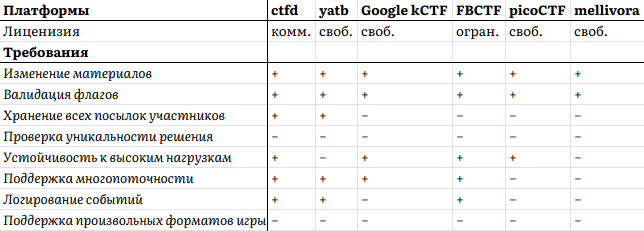
\includegraphics[width=0.9\textwidth]{inc/img/boards-table}
  \caption{Таблица 2.1. Сравнительный анализ наиболее популярных платформ для Jeopardy CTF}
  \label{fig:jeopardy}
\end{figure}

Существует множество программных продуктов, позволяющих проводить jeopardy -- CTF-соревнования: организаторам необходимо лишь собрать участников, разработать задания и загрузить их на готовую платформу.

Анализ наиболее популярных готовых проверяющих систем для Jeopardy CTF показал, что ни одна такая система не удовлетворяет всем необходимым требованям (табл. 2.1). Выборка состоит из трёх систем, наиболее популярных на ресурсе Github\cite{GithubCTFTag} по тегу «ctf board» (yatb, picoCTF, mellivora), а также трёх систем, которые используются для проведения наиболее популярных международных соревнований по статистике агрератора CTFTime.org\cite{CTFTime}.

\section{Генерация вариантов задач и их развёртывание}

Обычно размещают задачи и следят за их работоспособностью вручную — можно автоматизировать этот процесс. Задачи часто однотипны с инфраструктурной точки зрения: это или веб-приложения, или сервисы на сокетах, или сгенерированные автоматически файлы. Можно разработать систему, позволяющую декларативно описать, как устроена задача, и делегировать полномочия по её развёртыванию борде.

Это же поможет реализовать более защиту от списывания: генерировать каждой команде по своему собственному варианту задачи со своим собственным флагом. Даже если задача статическая (например, на криптографический анализ текста).

Реализовать такой механизм можно, реализовав программный интерфейс для запуска задач. Конфигурация конкретной задачи описывается на формальном языке.

Для развёртывания статических задач борде передаётся т.н. генератор — программа, криптографическими методами генерирующая флаг задачи для конкретного участника, условие и файлы-вложения, если они есть.

Для развёртывания динамических задач борде, помимо генератора, передаётся инструкция по запуску процесса, тому, на каком домене или адресе он должен быть доступен, и при каких условиях его необходимо перезапустить или остановить.

Генерация варианта задачи может оказаться ресурсоёмким процессом. Для таких случаем необходимо предусмотреть возможность предварительной генерации определённого числа вариантов, когда нагрузка на инфраструктуру минимальна (например, до начала соревнований) с кешированием результатов и распределением между участниками по мере их появления.

\subsection{Система, предоставляющая очным участникам программную среду для решения задач}

Каждому участнику на площадке предоставляется компьютер.

Программная среда компьютера должна быть пригодной для решения CTF-задач: нужен Linux с правами администратора (чтобы устанавливать своё ПО, изменять конфигурацию системы и т.п.).

Поскольку компьютеры не наши, жёсткий диск лучше не трогать.

Следовательно, среду лучше записывать на внешний загрузочный носитель — причём, участнику давать доступ к виртуальной машине, а в родительской ОС разместить инструменты прокторинга и провизии.

Использование виртуальной машины подразумевает наличие какого-то образа ОС. Поскольку это непринциаильный момент, можно предусмотреть возможность участника, при его желании, использовать свой образ ОС, а также поставлять универсальный «нейтральный» образ любого подходящего дистрибутива ОС Linux. Например, Kali Linux — наиболее распространённый дистрибутив, в комплекте поставки которого содержится большое количество инструментов для исследования уязвимостей.

Таким образом, можно сформулировать требования к функциональности такой системы.

\begin{figure}
  \centering
  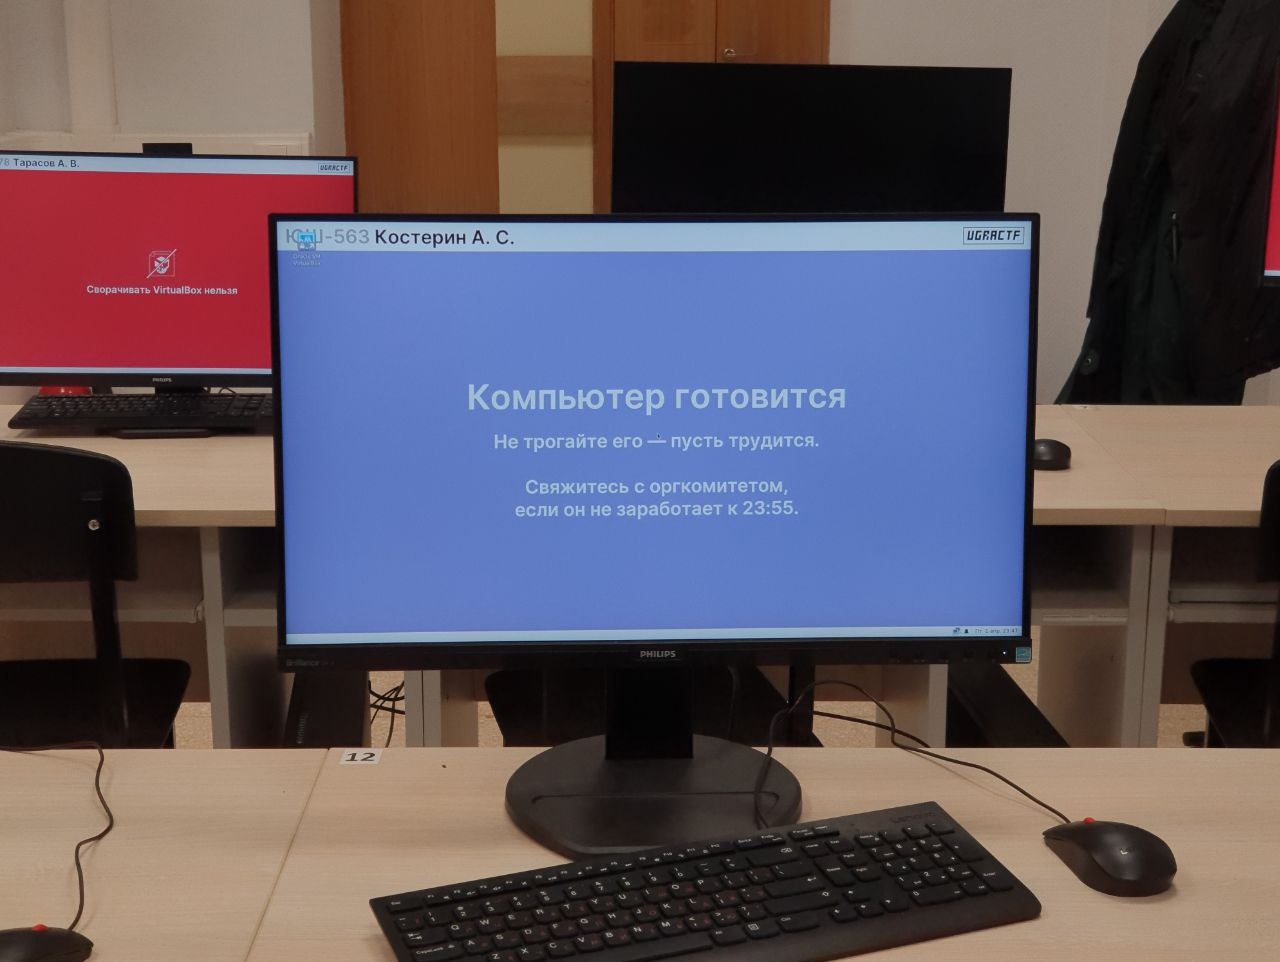
\includegraphics[width=0.7\textwidth]{inc/img/ugra-schoolos}
  \caption{Инициализация системы SchoolOS на соревнованиях Ugra CTF School 2022 в Долгопрудном}
  \label{fig:jeopardy}
\end{figure}

\begin{enumerate}
\item Автоматически разворачивается виртуальная машина с образом ОС, заблаговременно предоставленным участником через свой личный кабинет;
\item Все остальные приложения полностью изолируются от участника;
\item Реализованы элементы прокторинга: периодически с машины каждого участника собираются скриншоты, которые в перспективе планируется автоматически анализировать на предмет нарушения правил — там всё неочевидно, поскольку мы разрешаем пользоваться интернетом, но запрещаем любую внешнюю помощь и распространение условий задач;
\item Настраивается сетевой тоннель в общую игровую сеть;
\item Обеспечивается возможность удалённого доступа организаторов к любой машине;
\item Гарантируется невозможность модификации запущенной хост-ОС: её системных файлов, конфигурации ПО и пользователей с группами.
\end{enumerate}

Прокторинг:
\begin{itemize}
\item
  запись экрана;
\item
  контроль целостности ОС.
\end{itemize}

Провизия:
\begin{itemize}
\item
  участники могут работать в любой ОС, образ которой заблаговременно предоставят, либо в стандартом окружении Kali Linux (вариант по умолчанию);
\item
  конфигурация сети;
\item
  вывод на рабочем столе сведений об участниках («подписать», где чей компьютер);
\item
  возможность удалённого доступа к каждой машине для администрирования.
\end{itemize}




\section{Общая модель системы}

\subsection{Модель компьютерной системы}

\begin{itemize}
\item
  сервер жюри с бордой (веб-интерфейс, HTTPS);
\item
  сервер провизии и прокторинга (управление через SSH);
\item
  хранилище образов ВМ участников;
\item
  рабочие места участников.
\end{itemize}

\section{Модель угроз}

\subsection{Модель нарушителя}

Участник:
\begin{itemize}
\item
  может общаться в интернете
\item
  может обмениваться флагами с другими участниками
\item
  может обмениваться условиями задач с внешним миром
\item
  может атаковать инфраструктуру (в разных местах)
\end{itemize}

Организатор:
\begin{itemize}
\item может помогать участникам
\item может получить доступ к условиям задач
\item может не пресекать нарушения правил
\end{itemize}
